

\newcommand{\pdftitel}{Smarter Home}
\newcommand{\autor}{Andreas Rau}
\newcommand{\arbeit}{T-3300}

%----------------------------------------------------------------------------
% PREFERENCES
%----------------------------------------------------------------------------
\documentclass[
	12pt,
	a4paper,
	titlepage,
	oneside
]{article}			

%Seitengroesse
\usepackage[top=1in, bottom=1in, left=1in, right=1in]{geometry}
%\usepackage{fullpage}

%Exkurse
\usepackage{blindtext}

%Zeilenumbruch und mehr geht nur am MAC!!
\usepackage[activate]{microtype} 
\usepackage{lmodern}

% Zeichencodierung
\usepackage[utf8]{inputenc}
\usepackage[T1]{fontenc}

% Zeilenabstand
\usepackage[doublespacing]{setspace}

% Index-Erstellung
\usepackage{makeidx}

% Lokalisierung (englische Sprache)
\usepackage[american]{babel}

% Anführungszeichen 
%\usepackage[babel,german=quotes]{csquotes}
\usepackage{csquotes}

%tableen
\usepackage{tabularx}

% Spezielle Tabellenform fuer Deckblatt
\usepackage{longtable}
\setlength{\tabcolsep}{10pt} %Abstand zwischen Spalten
\renewcommand{\arraystretch}{1.5} %Zeilenabstand


%Matrix
\usepackage{multirow}


% Grafiken
\usepackage{graphicx}

% Mathematische Textsaetze
\usepackage{amsmath}
\usepackage{amssymb}

% Pakete um Textteile drehen zu können, oder eine Seite Querformat anzeigen kann.
%\usepackage{rotating}
%\usepackage{lscape}

% Farben
\usepackage{color}
\definecolor{LinkColor}{rgb}{0,0,0}
\definecolor{ListingBackground}{rgb}{0.92,0.92,0.92}
\definecolor{grey}{rgb}{.3,.3,.3}


% PDF Einstellungen
\usepackage[
	pdftitle={\pdftitel},
	pdfauthor={\autor},
	pdfsubject={\arbeit},
	pdfcreator={pdflatex, LaTeX with KOMA-Script},
	pdfpagemode=UseOutlines, 			% Beim Oeffnen Inhaltsverzeichnis anzeigen
	pdfdisplaydoctitle=true, 			% Dokumenttitel statt Dateiname anzeigen.
	pdflang=eng, 						% Sprache des Dokuments.
]{hyperref}

% (Farb-)einstellungen für die Links im PDF
\hypersetup{
	colorlinks=true, 					% Aktivieren von farbigen Links im Dokument
	linkcolor=LinkColor, 				% Farbe festlegen
	citecolor=LinkColor,
	filecolor=LinkColor,
	menucolor=LinkColor,
	urlcolor=LinkColor,
	bookmarksnumbered=true 				% Überschriftsnummerierung im PDF Inhalt anzeigen.
}

\usepackage{multicol}

% Hurenkinder und Schusterjungen verhindern
% http://projekte.dante.de/DanteFAQ/Silbentrennung
\clubpenalty=10000
\widowpenalty=10000
\displaywidowpenalty=10000


\usepackage{todonotes}					% for todos

% Quellcode
\usepackage{listings}
\lstloadlanguages{Java}
\lstset{
	language=PHP,            		% Sprache des Quellcodes
	numbers=left,           		% Zeilennummern links
	stepnumber=1,            		% Jede Zeile nummerieren.
	numbersep=5pt,           		% 5pt Abstand zum Quellcode
	numberstyle=\tiny,       		% Zeichengrösse 'tiny' für die Nummern.
	breaklines=true,         		% Zeilen umbrechen wenn notwendig.
	breakautoindent=true,    		% Nach dem Zeilenumbruch Zeile einrücken.
	postbreak=\space,        		% Bei Leerzeichen umbrechen.
	tabsize=2,               		% Tabulatorgrösse 2
	basicstyle=\ttfamily\footnotesize, % Nichtproportionale Schrift, klein für den Quellcode
	showspaces=false,        		% Leerzeichen nicht anzeigen.
	showstringspaces=false,  		% Leerzeichen auch in Strings ('') nicht anzeigen.
	extendedchars=true,      		% Alle Zeichen vom Latin1 Zeichensatz anzeigen.
	captionpos=b,            		% sets the caption-position to bottom
	backgroundcolor=\color{ListingBackground} % Hintergrundfarbe des Quellcodes setzen.
}

% Glossar
\usepackage[
	nonumberlist, 					%keine Seitenzahlen anzeigen
	acronym,    	  			 	%ein Abkürzungsverzeichnis erstellen
	section,     					%im Inhaltsverzeichnis auf section-Ebene erscheinen
	toc,          					%Einträge im Inhaltsverzeichnis
]{glossaries}

%bibliographie
%\usepackage[authoryear]{natbib}
%\usepackage{apacite}

\usepackage[backend=biber,date=short,maxcitenames=2,style=apa]{biblatex}
\DeclareLanguageMapping{american}{american-apa}

\addbibresource{literature.bib}


% Fussnoten
\usepackage[perpage, hang, multiple, stable]{footmisc}

% Titel, Autor und Datum
\title{\titel}
\author{\autorA}
\author{\autorB}
\date{\datum}



% Kopf und fußzeile
\usepackage{fancyhdr} 





% Ab jetzt können auch Umlaute verwendet werden
\newcommand{\titel}{Smarter Home middleware for SDPVnext and Apple Homekit}
\newcommand{\matrikelnr}{4186494}
\newcommand{\kurs}{TINF12A}
\newcommand{\datumAbgabe}{June 2015}
\newcommand{\firma}{IBM}
\newcommand{\firmenort}{Böblingen}
\newcommand{\abgabeort}{Stuttgart}
\newcommand{\studiengang}{Applied Computer Science}
\newcommand{\dhbw}{Baden Württemberg in Stuttgart}
\newcommand{\betreuer}{Jochen Burkhardt}
\newcommand{\zeitraum}{12 Weeks}

\makeglossaries
%
% vorher in Konsole folgendes aufrufen: 
% makeglossaries makeglossaries dokumentation.acn && makeglossaries dokumentation.glo
%

%
% Abkürzungen --> referenz, name, beschreibung
% Aufruf mit \gls{...} oder Kurzform mit \acrshort{...}
%

\newacronym{DSRC}{DSRC}{Dedicated Short Range Communications}
\newacronym{GPS}{GPS}{Global Positioning System}
\newacronym{GUI}{GUI}{Graphical User Interface}
\newacronym{IPS}{IPS}{Indoor Positioning System}
\newacronym{INS}{INS}{Indoor Navigation System}

% Glossareintraege --> referenz, name, beschreibung
% Aufruf mit \gls{...}
%
%\newglossaryentry{Glossary-entry}{name={Glossary-entry},plural={Glossary-entries},description={A Glossary describes different things in short words.}}




\newglossaryentry{Smart_City}{name={Smart City}, description={A Smart City is a settlement area where sustainable products, services, technologies, processes and infrastructures are developed with ecologic, social and economic aspects using highly integrated information and communication technologies. }}



\clearpage

\begin{document}
	%Todo
	\input{content/00todo}
	\clearpage
	
	% Deckblatt
	\begin{spacing}{1}
		\begin{titlepage}
	\begin{center}
		
\includegraphics[height=2.6cm]{images/dhbw.png}
	\end{center}
	\enlargethispage{20mm}
	\begin{center}
	  \begin{spacing}{2}
	  \vspace*{9mm}	{\Large\bf \titel }\\
	  \end{spacing}
	  \vspace*{8mm}	{\large\bf \arbeit}\\

	  \vspace*{17mm}	at Course of Studies \studiengang\\
	  \vspace*{3mm} 	at the Cooperative State University \dhbw\\
	  \vspace*{12mm}	by\\
	  \vspace*{3mm} 	{\large\bf \autor}\\
	  \vspace*{12mm}	\datumAbgabe\\
	\end{center}
	\vfill
	\begin{spacing}{1.2}
	\begin{tabbing}
		mmmmmmmmmmmmmmmmmmmmmmmmmm     \= \kill
		\textbf{Supervisor}              \>  \betreuer\\
		\\
		\textbf{\autor}\\
		Student ID, Course  \>  \matrikelnr, \kurs\\
		Company      \>  \firma, \firmenort\\
		
		
	\end{tabbing}
	\end{spacing}
\end{titlepage}

	\end{spacing}
	\clearpage
	
	% Erklärung
	\thispagestyle{empty}

\section*{Author's declaration}

\vspace*{2em}
Unless otherwise indicated in the text or references, this paper is entirely the product of my own scholarly work. This paper has not been submitted either in whole or part, for a degree at this or any other university or institution. This is to certify that the printed version is equivalent to the submitted electronic one.\\

Gemäß § 5 (2) der „Studien- und Prüfungsordnung DHBW Technik“ vom 18. Mai 2009.
Ich habe die vorliegende Arbeit selbstständig verfasst und keine anderen als die angegebenen Quellen und Hilfsmittel verwendet.
\vspace*{3em}\\
\abgabeort, \datumAbgabe\\
\begin{tabbing}
	mmmmmmmmmmmmmmmmmmmmmmmmmm     \= \kill


	\vspace*{4em}\\
	\rule{6cm}{0.4pt}
	\autor	



\end{tabbing}
	\clearpage

	% Abstract
	\pagestyle{empty}

\renewcommand{\abstractname}{Abstract}
\begin{abstract}

\textbf{Background:} In order to improve the efficiency of urban areas there is currently a movement heading to the Smart City. Buildings are a part of the Smart City where the social infrastructure has gained the need for reliable positioning systems. In this paper, a short summary of literature about social acceptance of innovations is given. Then different use cases of positioning systems in Smart Cities are collected and basic approaches for positioning systems are outlined. By comparing the different approaches guidance for future implementations is given.

\textbf{Concept:} In this paper a model for a positioning system working for the user and not for a third party is given. The variety of sensors the system relies on can be spitted into two fields - motions and radio-frequency sensors. While radio-frequency sensors are using the infrastructure motion sensors are part of the navigation device. 

\textbf{Conclusion:} Positioning systems are usefull for many of our daily activities but for all indoor usecases there are only a few concepts fullfilling the needs of accuracy and map matching. Our concept is an architecture combining both types of sensors with suitable algorithms and constraints. Our solution is based on an independent approach and therefore compliant with privacy by design.


\end{abstract}


	\clearpage
		
	\renewcommand{\thepage}{\Roman{page}}
	\setcounter{page}{1}
	\pagestyle{plain}

	% Inhaltsverzeichnis
	\begin{spacing}{1.1}
		\setcounter{tocdepth}{3}
		\tableofcontents
	\end{spacing}
	\clearpage
	
	% Abbildungsverzeichnis
	\cleardoublepage
	\phantomsection \label{listoffig}
	\addcontentsline{toc}{section}{List of figures}
	\listoffigures
	\clearpage
	
	% Abkürzungsverzeichnis
	% vorher in Konsole folgendes aufrufen: 
	%	makeglossaries makeglossaries dokumentation.acn && makeglossaries dokumentation.glo
	\printglossary[type=\acronymtype]
  	\cleardoublepage	
	
	\renewcommand{\thepage}{\arabic{page}}
	\setcounter{page}{1}
	
	\pagestyle{fancy} 
		
	\rhead{} \chead{\textcolor{grey}{\thepage}} \lhead{} 
	\lfoot{\textcolor{grey}{\datumAbgabe}} \cfoot{} \rfoot{\textcolor{grey}{Andreas Rau}} 
		
	\renewcommand{\headrulewidth}{0.2mm} 
	\renewcommand{\footrulewidth}{0.2mm} 
	\setlength{\headheight}{0mm}
	
	
	% Inhalt
	 \newpage
\section{Introduction}  % 8 - 12 Seiten

\subsection{Topic and Motivation} %includes current situation, trend and statement of the problem
	The term iot is around for more than two decades. The concept of a smart device being connected to the internet was realized by four students of the Carnegie Mellon University by modifying a coke vending machine to be able to report it's inventory and temperature in 1982 \parencite{cokeVendingMachineIoT}. Several companies have started their iot approaches among them Microsoft's "At work" and Novell's "Nest". The concept of iot became popular in 2002 when Paolo Magrassi introduced MIT's RFID and internet of things technology to the industrial and business world \parencite{E-Tagging}. The idea of identifying and connecting every device possible to control and manage them over a centralized computer has driven iot to todays understanding of smart devices \parencite{SmartObjects}. Smart Home is one application of iot. Being able to monitor and control the mechanical, electrical and electronic systems independent of your location offers new opportunities in terms of security and economization. As of 2014 smart home arrived at the average user by using the possibilities of smart phones to control your smart devices at home \parencite{IntroToHomeKit}. A lot of movement in the IoT and Smart Home sector is going on right now. Smart Home is a great opportunity for startups to develop innovating products that "push the boundaries of smart" \parencite{SmartHome-Techcrunch}. Established companies like Samsung and Google seek their dominance by acquiring these startups and integrate them into their own product line \parencite{SmartHome-Techcrunch}.

	%leitfrage: wie sieht ein smart home system aus, welches cross compatible und minimalistisch aufgebaut ist? Concept auf basis von apple homekit cross compatibility erweiterung mittels eines homebridges.

	%bekanntes bewertungssystem definieren und festlegen 
	\textbf{presentation of the problem}
		Current systems may have problems with connectivity or setup time and frequency \parencite{WhyIsMySmartHome}. However another big issue is cross compatibility when it comes to connect \textbf{all} of your home. It seems that hardly any company or vendor makes the approach to be able to connect or control devices of the competitors in a suitable way. This is the part where this thesis turns up the heat. The content of this thesis deals with smart home solutions and their cross compatibility. First of all basic definitions are clarified then theory is build up to emerge in a middleware solution which connects multiple vendors smart home solutions.

\subsection{Limitations}
	In the course of this bachelor thesis the middleware solution is limited to the guidelines of given systems. In other words the systems that have to be connected by a middleware are economically chosen by IBM. On one hand there is IBM SDPvNext which suits more or less a user management role for devices that are registered in the IoT Foundation which stores devices and their configurations in a database \parencite{FrankLeo}. At the time this paper is published SDPvNext will be integrated in the IoT Foundation Platform and be extended by an authentication layer \parencite{PatriziaGufler} but the two products are treated separately. \\

	On the other hand there is Apple HomeKit, a relatively new approach on smart home. Where Apple is relying on local databases for device information storage as well as waterproof communication encryption with multiple security layers \textcite{IntroToHomeKit} evaluated amongst other systems on the market in clause \textit{Measurements}. IBM SDPvNext is a more basic approach \textcite{FrankLeo}. This thesis will not cover explicit code explanations on the given solution nor specific programming language explanations, more describing the idea and the technique used to solve the given problem. However the code can be easily reproduced with the given explanations of what is done and some basic programming skills.\\

	Further the psychological significance of a home is not considered in this paper. Nevertheless the state as well as changes of a home has a strong influence on behavior, emotions and overall mental health \textcite{youngRefugees}.

\subsection{Goals}
	The goal of this thesis is to define measurements for a suitable smart home environment in the eyes of the user. Cross compatibility of vendors and devices as well as minimalism in the amount of extra hardware is valued. Further current systems are rated and two concepts of a middleware connecting multiple natively non connectable systems are developed and rated for further realization. The better solution is implemented and also rated.


	%which is connecting non HomeKit devices over IBM's IOT Foundation to the HomeKit database in order to manage them with iDevices and corresponding apps is developped. 
	%Due to the given constraints an implementation of the scheme is not needfull to call this thesis successfull.

\subsection{Tasks}
	The following tasks are written down in an artistic way which suits the creator of TEX Donald E. Knuth and its favor of describing programming as an art-form \parencite{Knuth}.
	At first terminology is declared to provide a consistent base for further argumentation. By specifying Smart Home measurements the solution gets its outlines. Thirdly a weighted overview of the functionality of every involved system and technology is given to provide the colors that will fill in the outlines. Last a solution is drawn with the technologies discussed earlier.

\pagebreak


	\section{Smart City and Indoor Positioning Systems} % 28-32 Seiten

\subsection{Definition of the Term Smart City} 
 
\subsubsection{What is a city?}
 
\subsubsection{\textit{Definition: City}}

\subsubsection{\textit{Definitions: Smart City}}


\subsection{Positioning in Smart Cities}\label{posInCS}

\subsubsection{Indoor Positioning System Use Cases}

\paragraph{Infrastructure Mode / Active (infrastructure) Sensor}

\paragraph{Independent Mode / Active Client}

\subsection{Social Acceptance of new Technologies}

\subsection{Basic Approaches for Indoor Positioning}

\subsubsection{Radio positioning strategies}

\subsection{Constraints}

\subsection{Sensor Fusion}

\subsection{Error correction and Filtering} \label{sec:error}

\subsubsection{Invalid Position Filter}

\subsubsection{Mask Filter} 

\subsubsection{Map Matching}

\pagebreak
	\section{Concept of discrete and reliable Indoor Positioning System}\label{concept} %28-32 Seiten

In the following sections we want to develop a trustworthy accurate and cost efficient indoor positioning system working in independent mode. To be able to do so the idea is to compare existing technologies on our three preconditions and learn from them. Therefore in the next section the measurements are defined followed by the comparison of the solutions worth considering. Then our concept is presented and discussed.   
 
\subsection{Measurements}
The three measurements we have chosen are directly concluded by the goals for our indoor positioning system. Trustworthiness is the only measurement which is not measurable directly but it is possible to derive measurements by more accurate defining trustworthiness.

\subsubsection{Trustworthiness}
Trustworthy means that data privacy is guaranteed. To ensure this in general systems which collect, use and handle personal data underlay restrictions by law. However, many companies as well as cities are interested in Data Mining. (Data Mining is of high importance for many decision making processes and getting even more important in times of Big Data.) Since we are talking about personal data like who was when where it is of high importance that this information cannot be tracked back to one specific person. Therefor only anonymized data is stored and analyzed. In the german Bundesdatenschutzgesetz § 3 Abs. 6 Data anonymization is defined as:
"Anonymisieren ist das Verändern personenbezogener Daten derart, dass die Einzelangaben über persönliche oder sachliche Verhältnisse nicht mehr oder nur mit einem unverhältnismäßig großen Aufwand an Zeit, Kosten und Arbeitskraft einer bestimmten oder bestimmbaren natürlichen Person zugeordnet werden können." \parencite{BDSG}

(translated from German)

"Anonymizing is manipulating personal Data in such a way that it is not, or only with a excessive effort in time, cost and manpower possible to match the single information - containing personal or factual coherences -  to one determined or determinable individual." \parencite{BDSG}

For the later measurement on trustworthyness we won't focus on the amount of data collected, but on the way it is, or could be collected. 
Thus a solution that collects only sparse data, but is able to determine the individuals is ranked less than one which collects a huge amount of data but is unable to determine the individual. 
For later comparison trustworthiness is roughly estimated in percent. 

\subsubsection{Accuracy}
Accuracy can be measured by exact values in three or two dimensional space. Given a variable $S$ containing the real positions and a variable $Z$ containing the assumed positions accuracy is defined as $\Delta = |S-Z|$. 

\subsubsection{Expected Cost}
 We define expected costs as cost for 10.000 square meters for one year including the implementation and additional fixed cost for services like a server providing constraint information.  Cost per square meter is only possible to determine for solutions requiring a special infrastructure like WiFi or iBeacons.  Solutions relying on infrastructure independent sensors (i.e. gyroscope and accelerator) are currently all assisted by constraint services.
 
Cost efficiency can be calculated by setting the measurements in relation to each other. Therefore we define that efficiency is an index without any bounds. Since trustworthiness is an estimated value in percent it could be used to influence the result directly by multiplication. For the accuracy smaller values are better. Thus the expected cost need to be divided by the accuracy. This leads to the function \\ $efficiency=(cost/accuracy)*trustworthiness$.

\subsection{Compared Existing Systems}
Under consideration of the Smart City context and the fact that we are focusing on systems working in independent mode  (i.a. because the infrastructure mode collects data without knowledge of the user) the following use cases of the previous collection are still covered.

\begin{enumerate}\itemsep0px
	\item General Indoor Navigation (with all its sub use cases)
	\item Personalized and Augmented Experiences
	\item People and Object tracking by active clients only
	\item Robotics
	\item Real Life Social Networks
	\item Geofences
\end{enumerate}

Not covered are: 
\begin{enumerate}\itemsep0px
	\item Proximity marketing, because our system is not about determining proximity, it is about determining a location.
	\item Location analytics, because every of the compared solutions could be extended by an analytic tool if the user agrees to forward his positions by various solutions - thus our later described solution. 
	\item People and Object tracking by active sensors which we expect to be the more favored by customers.
\end{enumerate}
	
To cover these use cases solutions currently on the marked and able to work in Smart Cities are compared. The list of solutions is provided in the next section.

\subsubsection{Systems Worth Considering}
As systems worth considering different solutions covering subsets of the covered use cases are taken into account. Since not every solution on the market can be considered, we tried to cover all use cases and all presented technologies on hardware site. Which algorithms are used in the background is often not published thus we wouldn't have been able to find enough solutions to compare the algorithms with at least a little bit of objectivity. The compared solutions are given in the next table:
\\

%http://www.directionsmag.com/entry/10-things-you-need-to-know-about-indoor-positioning/324602
\begin{singlespace}
\begin{tabularx}{14.65cm}{|p{2.5cm}|p{4cm}|p{6cm}|}\hline
	\textbf{Solution} & \textbf{Technologies} & \textbf{Use Cases}  \\ \hline
	Indoo.rs & Bluetooth 4.0  & Routing, Analytics and Proximity marketing \\ \hline
	Estimote & iBeacons & SDK for Distance, Proximity and Notification \\ \hline
	MazeMap & Flexible, but WiFi divided by Cisco is default & Interactive Indoor Map supporting indoor paths and positioning\\ \hline 
	infsoft & WiFi, Bluetooth 4.0 and internal sensors & Locating, Routing, Augmented Reality and Analytics \\ \hline
	Sailstech & WiFi, Bluetooth 4.0 and internal sensors & Locating, Routing \\ \hline
	Navizon & WiFi Fingerprinting (\& Active Beacons) & Locating, Routing \\ \hline
	Locata & Locata-GPS like & Locating, Routing \\ \hline
	ByteLight & LED light patters, Bluetooth, internal sensors & Routing, Proximity Marketing \\ \hline
	IndoorAtlas & Magnetic Flux & Locating, Routing \\ \hline
\end{tabularx}
\end{singlespace}

\subsubsection{The Comparison}
The following information was collected and estimated for the named solutions:

\paragraph{Indoo.rs} installed a Indoor navigation system at San Francisco International Airport (SFO) mentioned in the introduction \parencite{flySfo1}. The complete solution is built on Bluetooth 4.0 beacons. They do both proximity measurements and fingerprinting. If the corresponding app is installed in the navigation device it can work offline. If enabled real-time data collection is also provided. 
According to the Beacon calculator provided by indoo.rs for $10.000m^2$ around 150 Beacons would be needed \parencite{flySfo5}. (The following prices have been found on 7th May 2015: StickNFind: \$24 per beacon, shop.beaconinside.com: \$18 per iBeacon, shop.kontakt.io: \$20 per Beacon, bluesensenetworks.com: around \$20 per beacon. For our rough calculations 20\$ per beacon is assumed. And the small but full featured package is given with \$95 per month.
For one year minimal cost would be $150*\$20+12*\$95=\$4140$. An additional amount of development or adaption cost for an app and install the beacons at the customer site is not included.nOn their website the accuracy is given with up to 2 meters \parencite{flySfo5}.

The trustworthiness is hard to estimate since the solution is able to work offline but if enabled can provide real-time data collection and analytics. The last feature is optional and analyzing could be done with anonymized data. For the comparisson we assigned 90\% to tis value.


\paragraph{Estimote} installed a solution using iBeacons at London’s Heathrow airport and Britain’s Odeon Cinemas also mentioned in the introduction. Estimote itself is focusing on SDK development for routing, analytics \& proximity marketing. Since the SDK provides Distance measurements with trilateration localization can be implemented. Pricing is given with \$198 for 6 iBeacons on the website and an unknown volume discount is offered for larger quantity \parencite{estimote}. Assuming that the discount is around \$5 and still 150 beacons are needed the price would be $150*\$25=\$3750$ for the hardware plus additional individual cost on application development and installation. The accuracy is assumed with 2 meters the same as is for indoo.rs. 

Since the application programming would be done customized the trustworthiness can be taken as 100\%.


\paragraph{MazeMap} originaly a Campus Guide, from the NTNU Gloshaugen Campus in Norway and now available for enterprises \parencite{campusGuide1}, \parencite{mazemap}. MazeMap now is focusing on IndoorMaps that "are searchable, linkable, user-friendly and always up-to-date" \parencite{mazemap}.
For positioning they are writing "MazeMap can integrate with your Wi-Fi network or with other indoor location sources" \parencite{mazemap}. Since they are partnering with Cisco for Wifi positioning. Cisco itself uses a location aware WLAN Design with angle and distance based measurements and WiFi Fingerprinting for location determination \parencite{cisco}. 
To implement this service not necessarily new hardware is needed. For the pricing they are writing: "The basic bundle has an establishement cost of $\$0.15/m^2$. For feature add-ons, such as integration API and floorplan updates, pricing is giving upon request." \parencite{mazemap}. While the basic bundle does not include indoor positioning and indoor path. However assuming a doubled price for $10000m^2$ $\$3000$ and again plus additional individual cost on application development and installation.

Since the positioning itself is not part of this solution and the map is able to work with both independent and infrastructure mode a statement on trustworthiness is not possible. 

This solution is still in the list because MazeMap delivers a key element of every positioning systems and the map could be used for precise Map Matching. However it is not listed below because it could be linked to every solution, has no fixed accuracy, cost or trustworthiness. (Deep Map SDK and Visioglobe (European leader) are alternatives to MazeMap. Even Open Streetmap now offers Indoor Mapping.) 

\paragraph{infsoft} offers a solution in infrastructure mode and one in independent mode. The one in independent mode uses WiFi and internal sensors (gyroscope etc.) which can optionally be enhanced by Bluetooth Beacons. The accuracy is advertised wit 1m only, and there is no word on pricing on their website. 
In independent mode trustworthiness is guarantied accorting to their statement "The application periodically transmits the current position to the server, so that all smartphones using the application can be tracked. No personal data is captured, so that infsoft Indoor Location Analytics can be used in compliance with data protection regulations." \textcite{infsoft}. In infrastructure mode the devices can be tracked without any knowledge of the customer. In both cases the tracked person does not have any choice or does not even know that he is tracked. This fact reduces the trustworthiness for us to 70\%.

\paragraph{Sailstech} is a public project. The provider of a solution using Sailstech is completely free in the effort it invests. The softwaretools to use however are fixed: JOSM, SAILS MRE, BuildNGO and the SAILS SDK. The development costs, accuracy and trustworthiness for a project with Sailstech will highly depend on the goals of the project. Thats why we decided to not include the solution in the table below. 

\paragraph{Navizon} can be seen as direct competitor of infsoft. They are also providing positioning in infrastructure as well as independent mode. In independent mode accuracy is given with below 1m for iOS and Android and about 3m for other OS \parencite{navizon}. The solution uses WiFi fingerprinting as main technology for positioning \parencite{navizon}. The decision if the determined location is transmitted to an analyzing server or not can be made during application development. Therefore trustworthiness is high and the costs are again depending on the use case specifications. In Infrastructure Mode Active Navizon Beacons can determine the location of every WiFi enabled device - but this is not of importance for the comparison. 

\paragraph{Locata} invented its own GPS like technology "that creates terrestrial networks that function as a 'local ground-based replica' of GPS-style positionin" \parencite{locata}. Locata is suitable for wide area positioning system, but still does work inside due to a received signal strength of $-84 dBm$ at $10 km$ and $-64 dBm$ at $1 km$ from the LocataLite compared to the strongest GPS satellite signal of $-125 dBm$ \parencite{locata}.
This technology thus would be suitable to be installed at a whole urban area, but special receivers are needed. The potential of this technology are high if the major smartphone and GPS manufacturers consider to implement Locata receivers. The trustworthiness of this solutions is as high as it is for GPS - which is $100\%$ - because only receivers are able to locate themselves. 

Locata is a big opportunity for cities and even states to improve existing positioning systems and making indoor positioning in all buildings available at once. However such a project does not add any value to a cities infrastructure until receivers are not implemented into the commonly used devices.  

\paragraph{ByteLight} is combining light patterns with bluetooth 4.0 and internal sensors. The light patterns increase the accuracy reached by bluetooth only solutions to less than one meter. In addition to all the other solutions the front camera needs to be enabled during positioning \parencite{bytelight}. Trustworthiness is again could be a problem. The ByteLight platform is designed for personalized proximity marketing in the focus. Therefore the sharing of personalized data is one goal and trustworthiness would depend on how the data is stored. We decided to assign only 50\% of trustworthiness to this solution. 

\paragraph{IndoorAtlas} is focusing on magnetic flux and providing a cloud based solution. The SDK they provide enables the development of an indoor navigation app with three steps: At first the maps are uploaded to the IndoorAtlas Cloud, the IndoorAtlas app is used to record a magnetic flux map and afterwards the own app can be developed \parencite{indooratlas}.
Since the use case is not given or limited by the SDK the trustworthiness won't be causing any problems and pricing starts at \$99 per month for use of the cloud of IndoorAtlas.
\\
\\
Finally a comment to the \textbf{In-Location Alliance}, a cooperation between more than 20 members with the goal to accelerate indoor position solutions. 
This alliance announced three winners of a best use case contest 2014. The winners are indoo.rs with the San Francisco International Airport project, infsoft and vodafone for a solution at vodafones campus in Düsseldorf and iMap as well as Sailstech with a solution at the largest station in Taiwan - Taipei Railway Station \parencite{inLocation}. 

\begin{singlespace}
\begin{tabular}{|p{2.0cm}|p{2cm}|p{2.0cm}|p{2.0cm}|p{3.5cm}|} \hline
	\textbf{Solution} & \textbf{Accuracy} & \textbf{Costs $10000m^2$} & \textbf{Trustw.} & \textbf{Efficiency} \\ \hline
	Indoo.rs & 2m & \$4140 + \$x & 90\% & $e=((4140 + x)/2)*0.9$ \\ \hline
	Estimote & 2m & \$3750 + x \$& 100\% & $e=((3750 + x)/2)*0.9$ \\ \hline
	infsoft & 1m  &	\$x & 70\% & $e=x*0.7$ \\ \hline
	Navizon & 1m & \$x & 100\% & $e=x*1$ \\ \hline
	Locata & 0.1m & \$y & 100\% & $e=10*y$ \\ \hline
	ByteLight & <1m & \$x & 70\% &  $e>x/2$ \\ \hline
	IndoorAtlas & 2m &  \$1200 + z & 100\% & $e=z/2$ \\ \hline
\end{tabular}
\end{singlespace}

\subsubsection{The Winner}
Assuming $x$ to be high the range of costs for a solution is not as much influenced by the technologies as it is by the use case. We expect the overall costs for a Locata solution ($y$) much more expensive than for every other solution. However the average cost per square meter can be much less than for a single building or campus solution. So far this is only speculation and we will focus on solutions suitable for implementation not to far in the future. Assuming that the implementing team would always be the same ($x$) - the highest efficiency is reached by Navizon.
Only IndoorAtlas is expected to be cheaper since the setup using the SDK is done by using only three simple steps without any special hardware needed and the software is provided for free. 

Summarizing it is remarkable that most of the solutions are hybrids and use different sensors to calculate the position. WiFi and Bluetooth based positioning is used by the most solutions. The fact that fingerprinting can be achieved using manual fingerprinting, additional infrastructure or crowdsourcing - relying on users willing to share sensitive sensor and location information - is one big disadvantage of all these solutions \parencite{sail}. (A new technology in development using round trip signal propagation (Time-of-Flight) could possibly be a solution to this problem for WiFi \parencite{sail}.) The alternative to use light patters is only applicable in special use cases where the navigation device can be assumed to have a camera with a clear view to the ceiling.


But before we start designing our own system we decided to run some experiments to test some hypothesis regarding single positioning technologies.

\subsection{Preliminary Consideration of Experiments}
The two big competitors indoo.rs and estimote are both using iBeacons. While indoo.rs is using both fingerprinting and proximity measurements estimote is focusing on proximity measurements. Due to this we decided to make some experiments to decide which method to use. 

Then there is IndoorAtlas mainly relying on Magnetic Flux measurements. The question which popped up in our minds was: Is it possible to locate a device inside a environment with a little amount of metal? 

In the following section three experiments to answer the design questions are described.

\subsubsection{Proximity measurements with iBeacons}

\paragraph{Hypothesis: }
It is better to focus on Bluetooth proximity measurements then fingerprinting. 

\paragraph{Experiment design: } 
In our test environment we set up two Bluetooth beacons as shown in figure \ref{fig:positionsBea}. The proximity will be measured based on signal strength in all the 20 marked points. The shown walls and landmarks are barriers for the signals. 

If the results will show that the measured distances are highly influenced by these barriers we could assume that proximity measurements are not the way of choice. (Proof by contradiction.)

\begin{figure}[h]
	\centering
		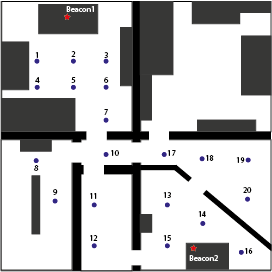
\includegraphics[width=.4\textwidth]{images/floorplan2ndf+positions.png}
	\caption{20 positions for measurements in our test environment ($9.5m\times 9.5m$).}
	\label{fig:positionsBea}
\end{figure}

\paragraph{Evaluation: } 
In figure \ref{fig:distaceBea1} the measured values of \textit{Beacon 1} are shown for the 20 points. In figure \ref{fig:distaceBea2} the measured values of \textit{Beacon 2} are shown for the 20 points. 


\begin{figure}[h]
	\centering
		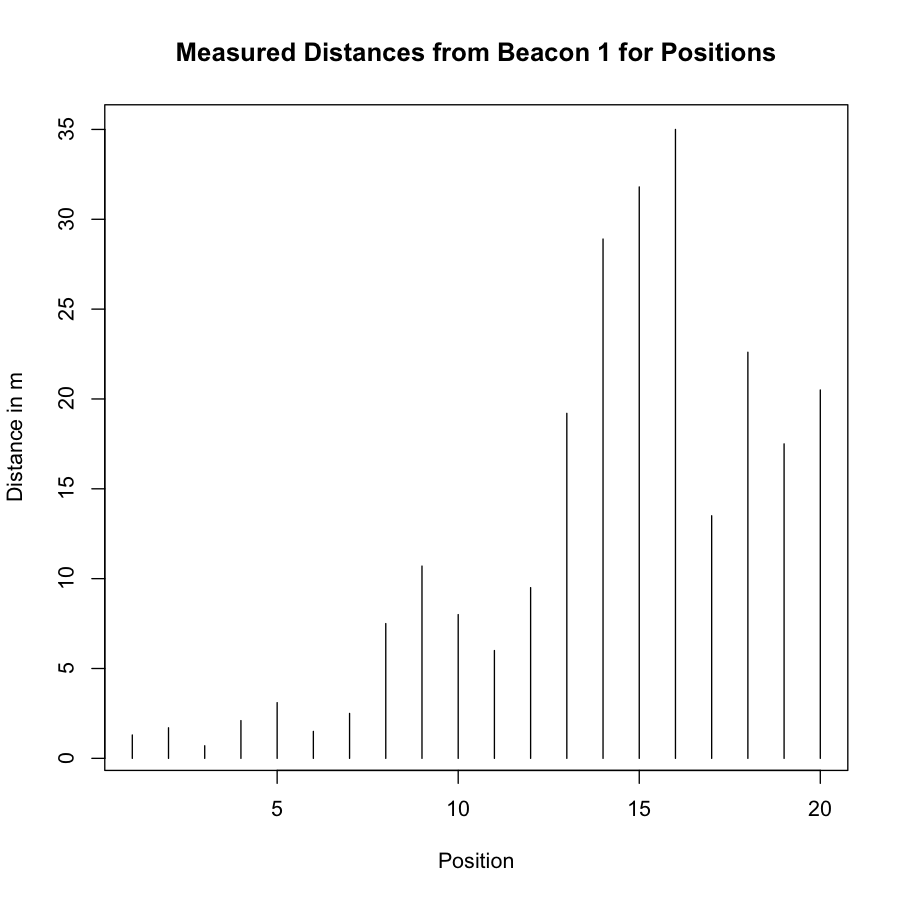
\includegraphics[width=.5\textwidth]{images/distaceBea1.png}
	\caption{Measured distances from Beacon 1 for the 20 locations}
	\label{fig:distaceBea1}
\end{figure}


As we can observe the measured values are up to $30m$ in an $9.5mx9.5m$ environment. This already shows that direct distance measurements are not very accurate. In more detail we can observe for \textit{Beacon 1} that the measured distance at position 9 is higher than on position 12 while the bee-line is shorter for position 9. 

\begin{figure}[h]
	\centering
		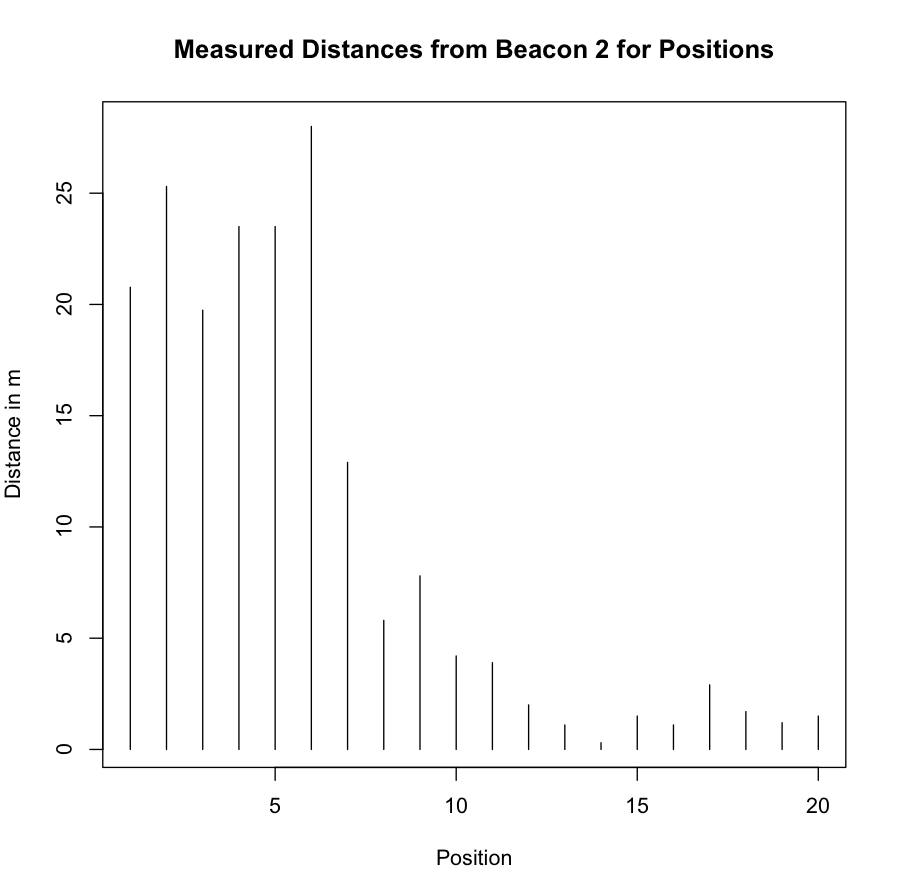
\includegraphics[width=.5\textwidth]{images/distaceBea2.png}
	\caption{Measured distances from Beacon 2 for the 20 locations}
	\label{fig:distaceBea2}
\end{figure}

However we are able to observe that the values are highly depending on the barriers and that there are individual combinations of the values from the two beacons. Due to this fact a fingerprinting map is possible with only two beacons. This leads to the next experiment where we try to proof that the fingerprinting map is the method of choice. 

\paragraph{Hypothesis: } 
It is better to focus on Bluetooth fingerprinting then on proximity measurements. 

\paragraph{Experiment design: } 
For a proof by contradiction - to show that fingerprinting is not better than direct proximity measurements we use the weak point of the fingerprinting map. The fingerprinting map assumes a static environment. Only if in every point in time at a specified location the measurements will have nearly the same values as stored in the map they could be matched.

Thus we need to show that a simple dynamic change will adulterating the results to much for a fingerprinting map. The simplest dynamic change we can assume is the body of the person navigating through the environment. 

For this experiment we used only one Beacon placed in a way that a direct path for measurement is possible and made measurements on distances $1m$, $5m$ and $8m$. For every distance we collect 10 measurements for the direct path and 10 with a body between Beacon and the receiving device. 

In figure \ref{fig:proxWithB1} the three points of measurement are marked. 

\begin{figure}[h]
	\centering
		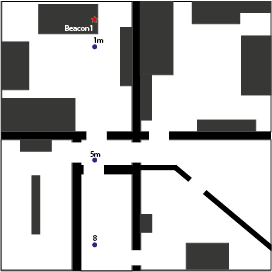
\includegraphics[width=.4\textwidth]{images/floorplan2ndf+normung.png}
	\caption{3 Distance measurements with a direct path.}
	\label{fig:proxWithB1}
\end{figure}

\paragraph{Evaluation: }
 
 In figure \ref{fig:proxWithB1} the boxplots for the measurements at the different positions are shown. Always at first the measurement without a barrier and the second one with a body as barrier. 

\begin{figure}[h]
	\centering
		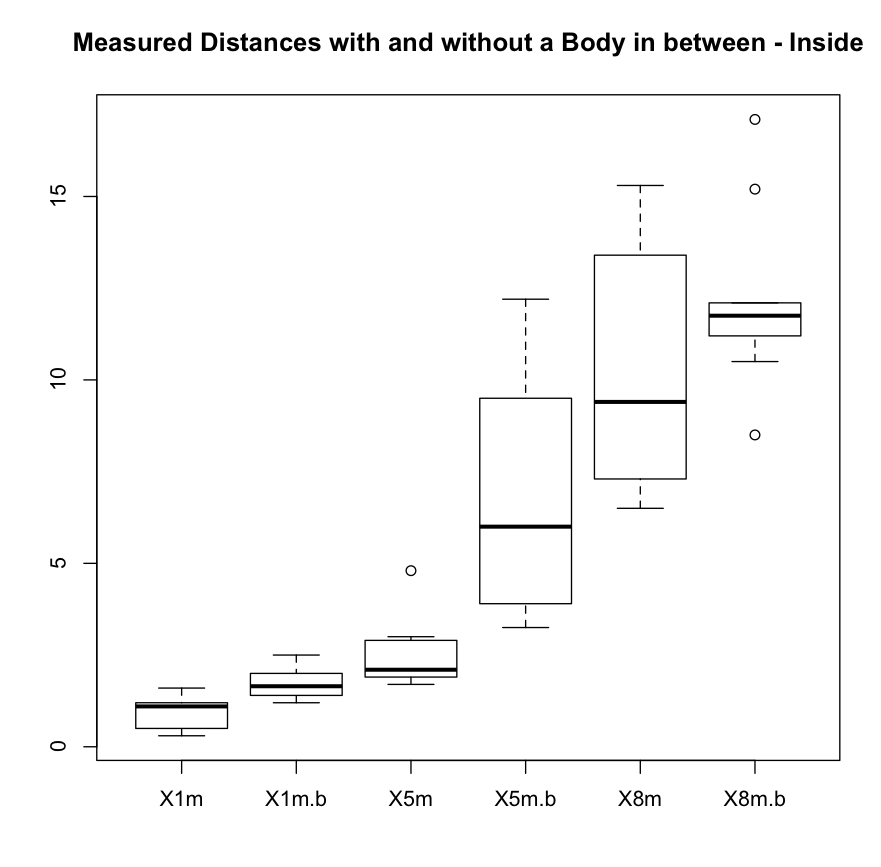
\includegraphics[width=.5\textwidth]{images/insideProx.png}
	\caption{Boxplots of proximity measurements with and without a body in between (Inside).}
	\label{fig:proxWithB1}
\end{figure}

 If we combine the measurements with and without barrier we have a maximum difference above 10m (for mean values still 4m). This already shows that even fingerprinting maps could not be used to determine a accurate position. 

 Surprisingly the diffusion rate of the measurements grows with the distance except for the last measurement (at 8m distance with barrier). Our assumption was that the reflection of the signal results in multi-path measurements for the higher distances, which would explain the higher diffusion rate. For position 3 the body maybe screening-off  a lot of possible path which results in a lower diffusion rate (with outliers) again. 
 However we decided to explain the effect by a third experiment.  

\paragraph{Experiment design: }
To avoid refections and therefor multi path measurements we decided to repeat our measurements outside on wide grassland. 
Again we measured at a distance of $1m$, $5m$ and $8m$ one time with and the second time without a body as barrier.

\paragraph{Evaluation: }

The results in figure \ref{fig:proxOutside} show that the variance does not grow as much as in the experiment before. Even more the variance grows with the barrier more than with the distance. The theory that the multipath effect caused the big variance fits to these results. This leads to the assumption that the most of the measurements are direct path signals which have been evaluated. Then the measured distance for 5m with barrier is higher than for 8m without body, and the measurement for 8m with barrier is far above 20m while it was below 15m indoors. Which fits to our theory again.

\begin{figure}[h]
	\centering
		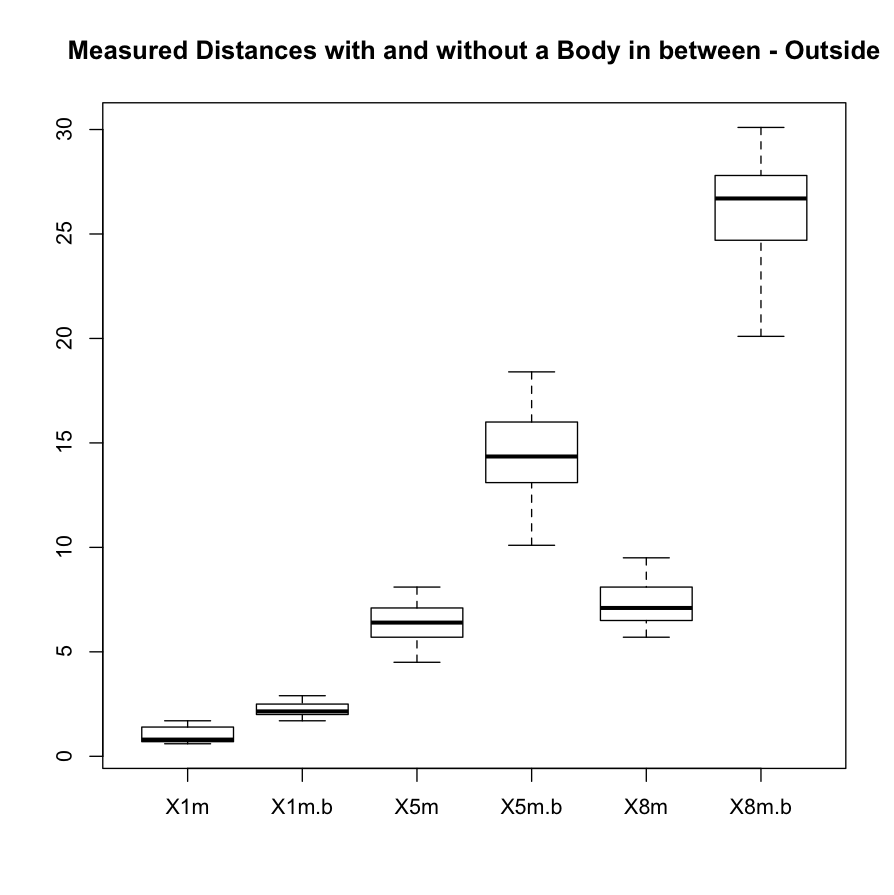
\includegraphics[width=.5\textwidth]{images/outsideProx.png}
	\caption{Boxplots of proximity measurements with and without a body in between (Outside).}
	\label{fig:proxOutside}
\end{figure}

\paragraph{Conclusion of Beacon Experiments: }
Neither proximity measurements nor fingerprinting map are providing results beyond doubt. The reflection rate and possible multipath measurement can highly influence measurements if no direct path is given. Even the position of the person navigating through an environment can adulterate the measure signals. 

These results show that a positioning system cannot trust absolute values. Only the deltas between signal strengths should be taken into account. To assure measurement deltas resulting of dynamic changes like a person passing the signal path wont affect the positioning evaluation of internal sensors will help out. 

However a combination of proximity and fingerprinting will be the best choice for our system.

\subsubsection{Magnetic flux in a house without steel}
At the beginning of this chapter we already denoted the Question: "Is it possible to locate a device inside a environment with a little amount of metal using magnetic flux?". We assume that the system IndoorAtlas sells is working in the most of the offices and public buildings having a lot of metal in it. However in a smart city there may be places with less steel. 

\paragraph{Hypothesis: } It is possible to locate a device inside a environment with a little amount of metal using magnetic flux.

\paragraph{Experiment design: } 
For this experiment we use the same test environment (inside of a wooden building). Since IndoorAtlas is providing a free iOS app for Development we just used this app. After downloading the app we needed to upload our indoor map into the IndoorAtlas Cloud. Then for calibration we needed to place a path on the map and then walk along this path in an constant speed. After doing so for half an hour we assumed to have a reliable map. We tested the map using again predefined test path. 
For out own tests we then tried to locate ourself while walking through the mapped area.

\paragraph{Evaluation: }
In figure \ref{fig:magneticX} the real position versus the measured position is shown for four situations.

\begin{figure}[h]
	\centering
		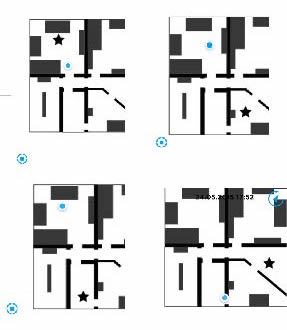
\includegraphics[width=.6\textwidth]{images/experiments/magnetic.jpg}
	\caption{The real position (star) versus the measured position (dot).}
	\label{fig:magneticX}
\end{figure}

The test results partly contradict our hypothesis. In this small area the possible paths should have been a small set. However the positioning failed. Therefore we cannot assume that magnetic flux is a feasible solution in all environments.

\paragraph{Conclusion: }
This experiment shows that the positioning does not work very well in our test environment. We conclude that the magnetic flux measurement should only influence the result in an metal full environment. The later described filter combining different sensor data should take this into account. Even more the magnetic flux map shows that there are no individual magnetic flux values allowing us to find a concrete position on a map. It is more a magnetic flux path - the measurements taken during some steps give magnetic flux changes characteristic for an specific area. 
In case of large buildings there will be steel graders influencing the magnetic flux much more. However it could happen that these steel graders are placed all in fixed distances resulting in self-repeating magnetic flux patterns. 
Altogether we can say that we are able to use Bluetooth to determine a rough absolute position and magnetic flux measurements to find the most likely path of movement (and thus position) inside this area. Since the results of the Bluetooth experiments show that the absolute position will be a very rough one. 

Now we take a short look at Wifi fingerprinting and internal sensor data in praxis. 

\subsubsection{WiFi Fingerprint}
Only a short look at for different WiFi signals in the test environment in figure \ref{fig:wifiTest} shows that determining absolute positions using WiFi won't be a big problem if there are enough access points in the area. 


\begin{figure}[h]
	\centering
		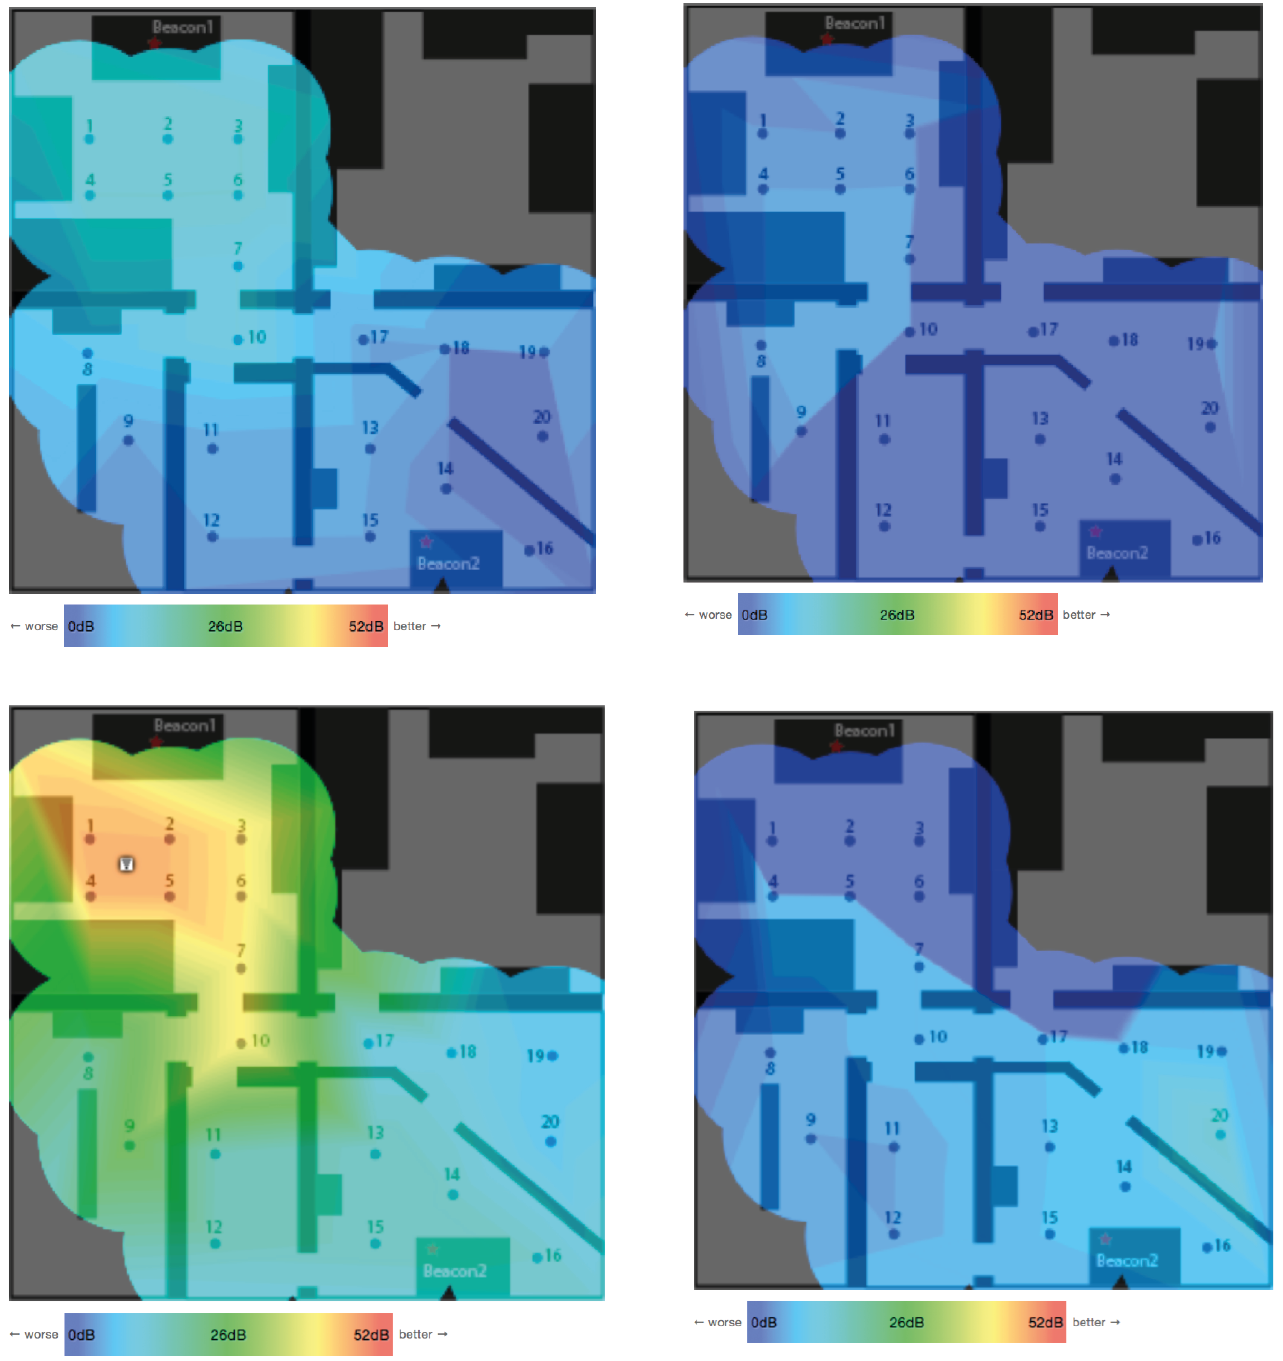
\includegraphics[width=.6\textwidth]{images/wifi.png}
	\caption{Four fingerprint maps of WiFi signals in the test environment.}
	\label{fig:wifiTest}
\end{figure}

Since not all WiFi signals have the same source the combination of at least three Access Points will enable a rough absolute positioning comparable to Bluetooth. 

\subsubsection{Internal Sensors}
None of the above methods could enable a accurate and stable service of positioning. However a rough absolute positioning is possible using beacons and WiFi. In these rough determined areas which can be assumed being reliable magnetic flux measurements can be used to state more precisely which area is the most likely one.

However to enable accurate positioning the evaluation of internal sensors is the best chance. To just show that a accurate positioning is possible we present the sensor data for different movements. 

At first a simple rotation. The rotation can be observed very accurate using the magnetometer, since it can be used to determine the absolute alignment to the magnetic field of the earth. In figure  \ref{fig:rotation} a horizontal rotation is shown. The rotation is represented in sinus curves. 

\begin{figure}[h]
	\centering
		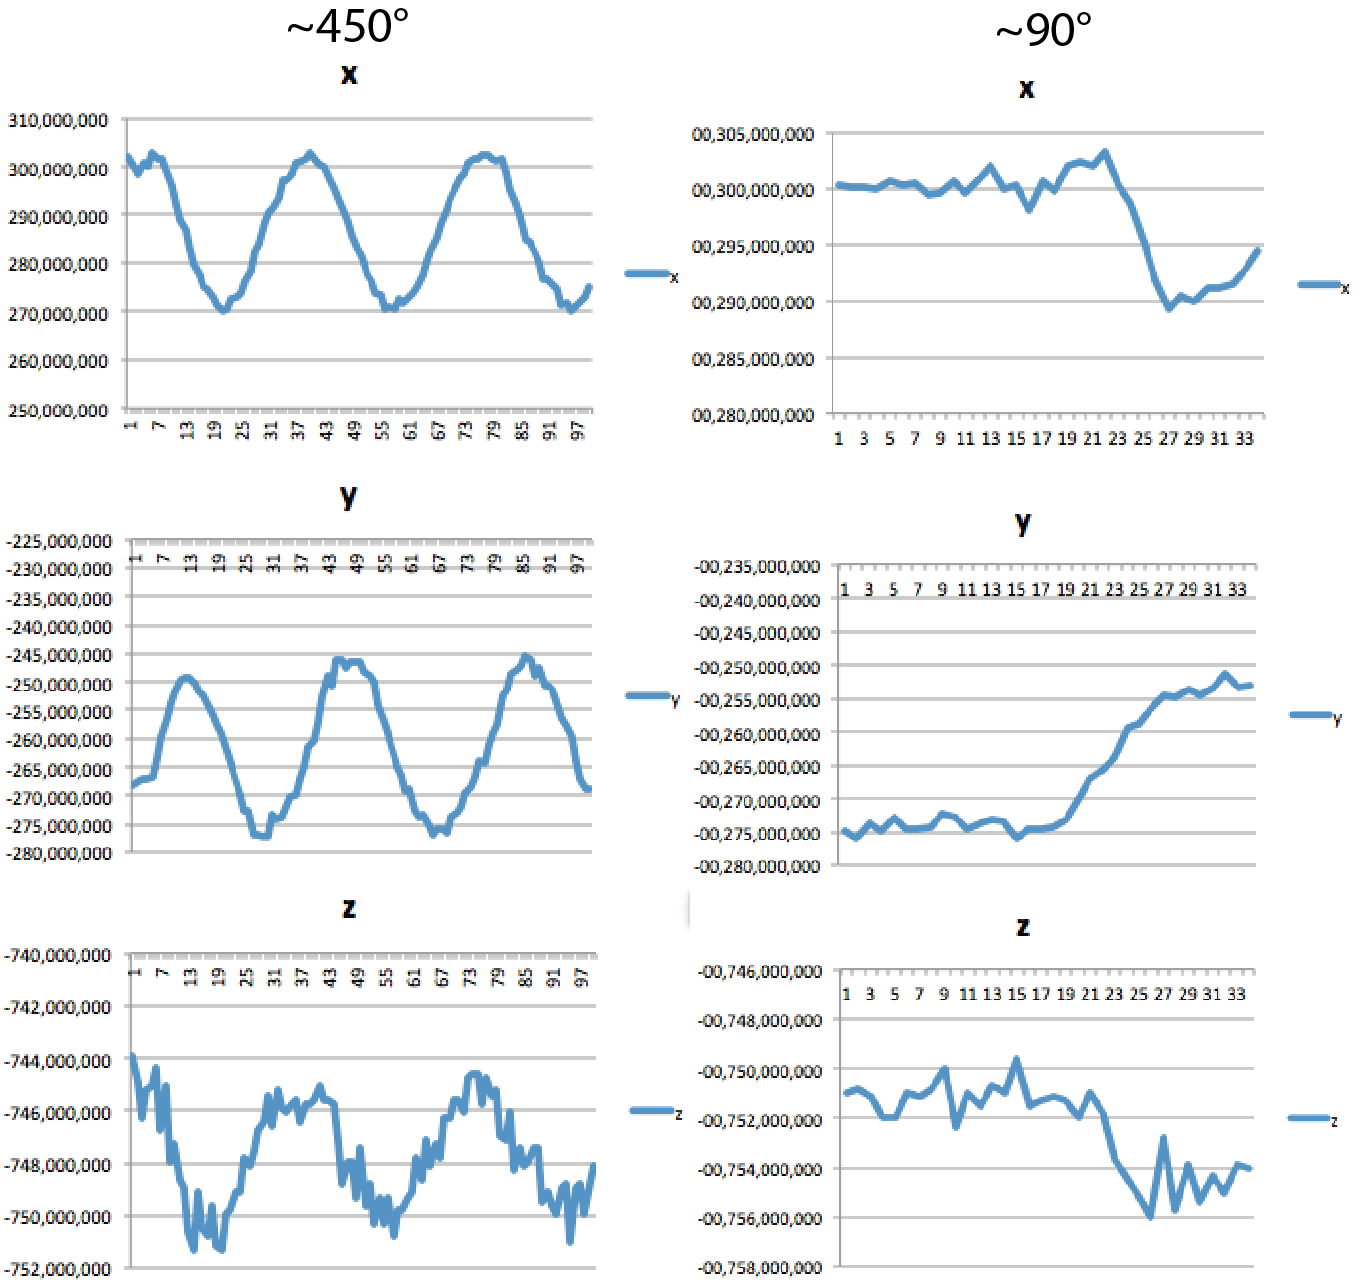
\includegraphics[width=.6\textwidth]{images/experiments/rotation.png}
	\caption{Measurements of the magnetometer for two different rotations.}
	\label{fig:rotation}
\end{figure}

Simple steps are shown in figure \ref{fig:steps}. They can easily count by finding all local maximum and minimum values. 


\begin{figure}[h]
	\centering
		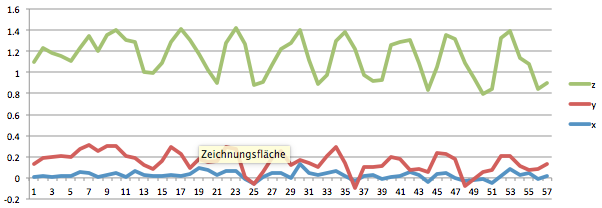
\includegraphics[width=.6\textwidth]{images/experiments/steps.png}
	\caption{Measurements of the accelerometer for steps on a straight line.}
	\label{fig:steps}
\end{figure}

In figure \ref{fig:edge} both movements are combined by going around an edge. We can observe the steps in the measurements of the accelerometer and are able to see the rotation in the measurements of the gyroscope and the accelerometer. 

\begin{figure}[h]
	\centering
		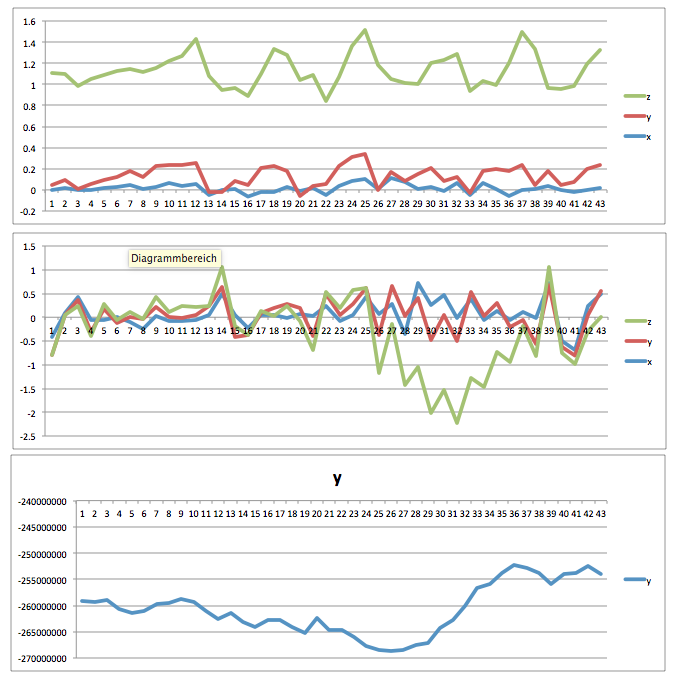
\includegraphics[width=.6\textwidth]{images/experiments/edge.png}
	\caption{Measurements of the accelerometer (1), gyroscope (2) and magnetometer in y-axis (3) are shown for going around an edge.}
	\label{fig:edge}
\end{figure}

Even if these measurements can be interpreted easily there are situations where they can by misleading. For example measurements of the accelerometer, gyroscope and magnetometer measurements for going around an edge are very similar to rotating the phone while walking (visible in figure \ref{fig:rotateWhileWalking}).

\begin{figure}[h]
	\centering
		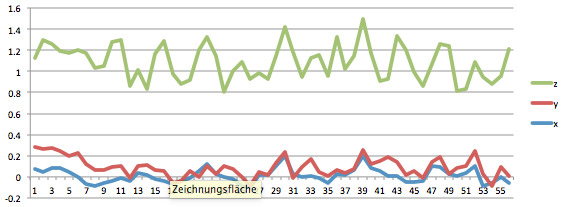
\includegraphics[width=.6\textwidth]{images/experiments/stairs.png}
	\caption{Measurements of the accelerometer going stairs up.}
	\label{fig:stairs}
\end{figure}

\begin{figure}[h]
	\centering
		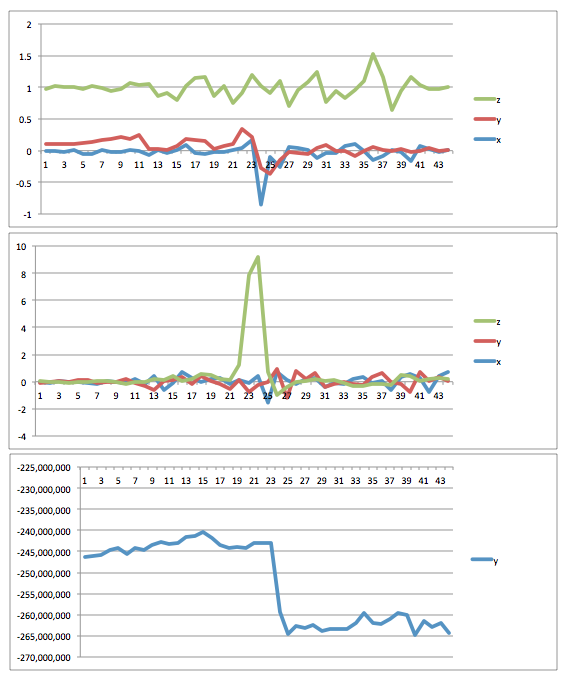
\includegraphics[width=.6\textwidth]{images/experiments/rotateWhileWalking.png}
	\caption{Measurements of the accelerometer (1), gyroscope (2) and magnetometer in y-axis (3) are shown for rotating the phone while walking a strait line.}
	\label{fig:rotateWhileWalking}
\end{figure}

Another example are stairs (see figure \ref{fig:stairs}) which are very similar to regular steps. Therefore the barometer will hopefully clarify the situation. Unfortunately we have not been able to make an experiment with an barometer. 



However this background knowledge is now applied to our own system design.


\pagebreak
\subsection{The Concept} 
The concept of the system architecture we are designing had the goal for a high overall efficiency. We decided to use a modular approach for the solution to make sure that different Smart City needs can be fulfilled. To guaranty trustworthiness and reach social acceptance we suggest to stick to the concept of the MIT and give the user ability to choose which and how much information he want to share. 

In the next steps we explain our decision for different technologies presenting the model and discuss the advantages and disadvantages of this model.

The model contains three main elements: Sensors, Constraints and Filters. Clients could just load the constraints from one application server or they are already included into the app before they are applied through filters to the sensor data. 

\begin{figure}
	\centering
		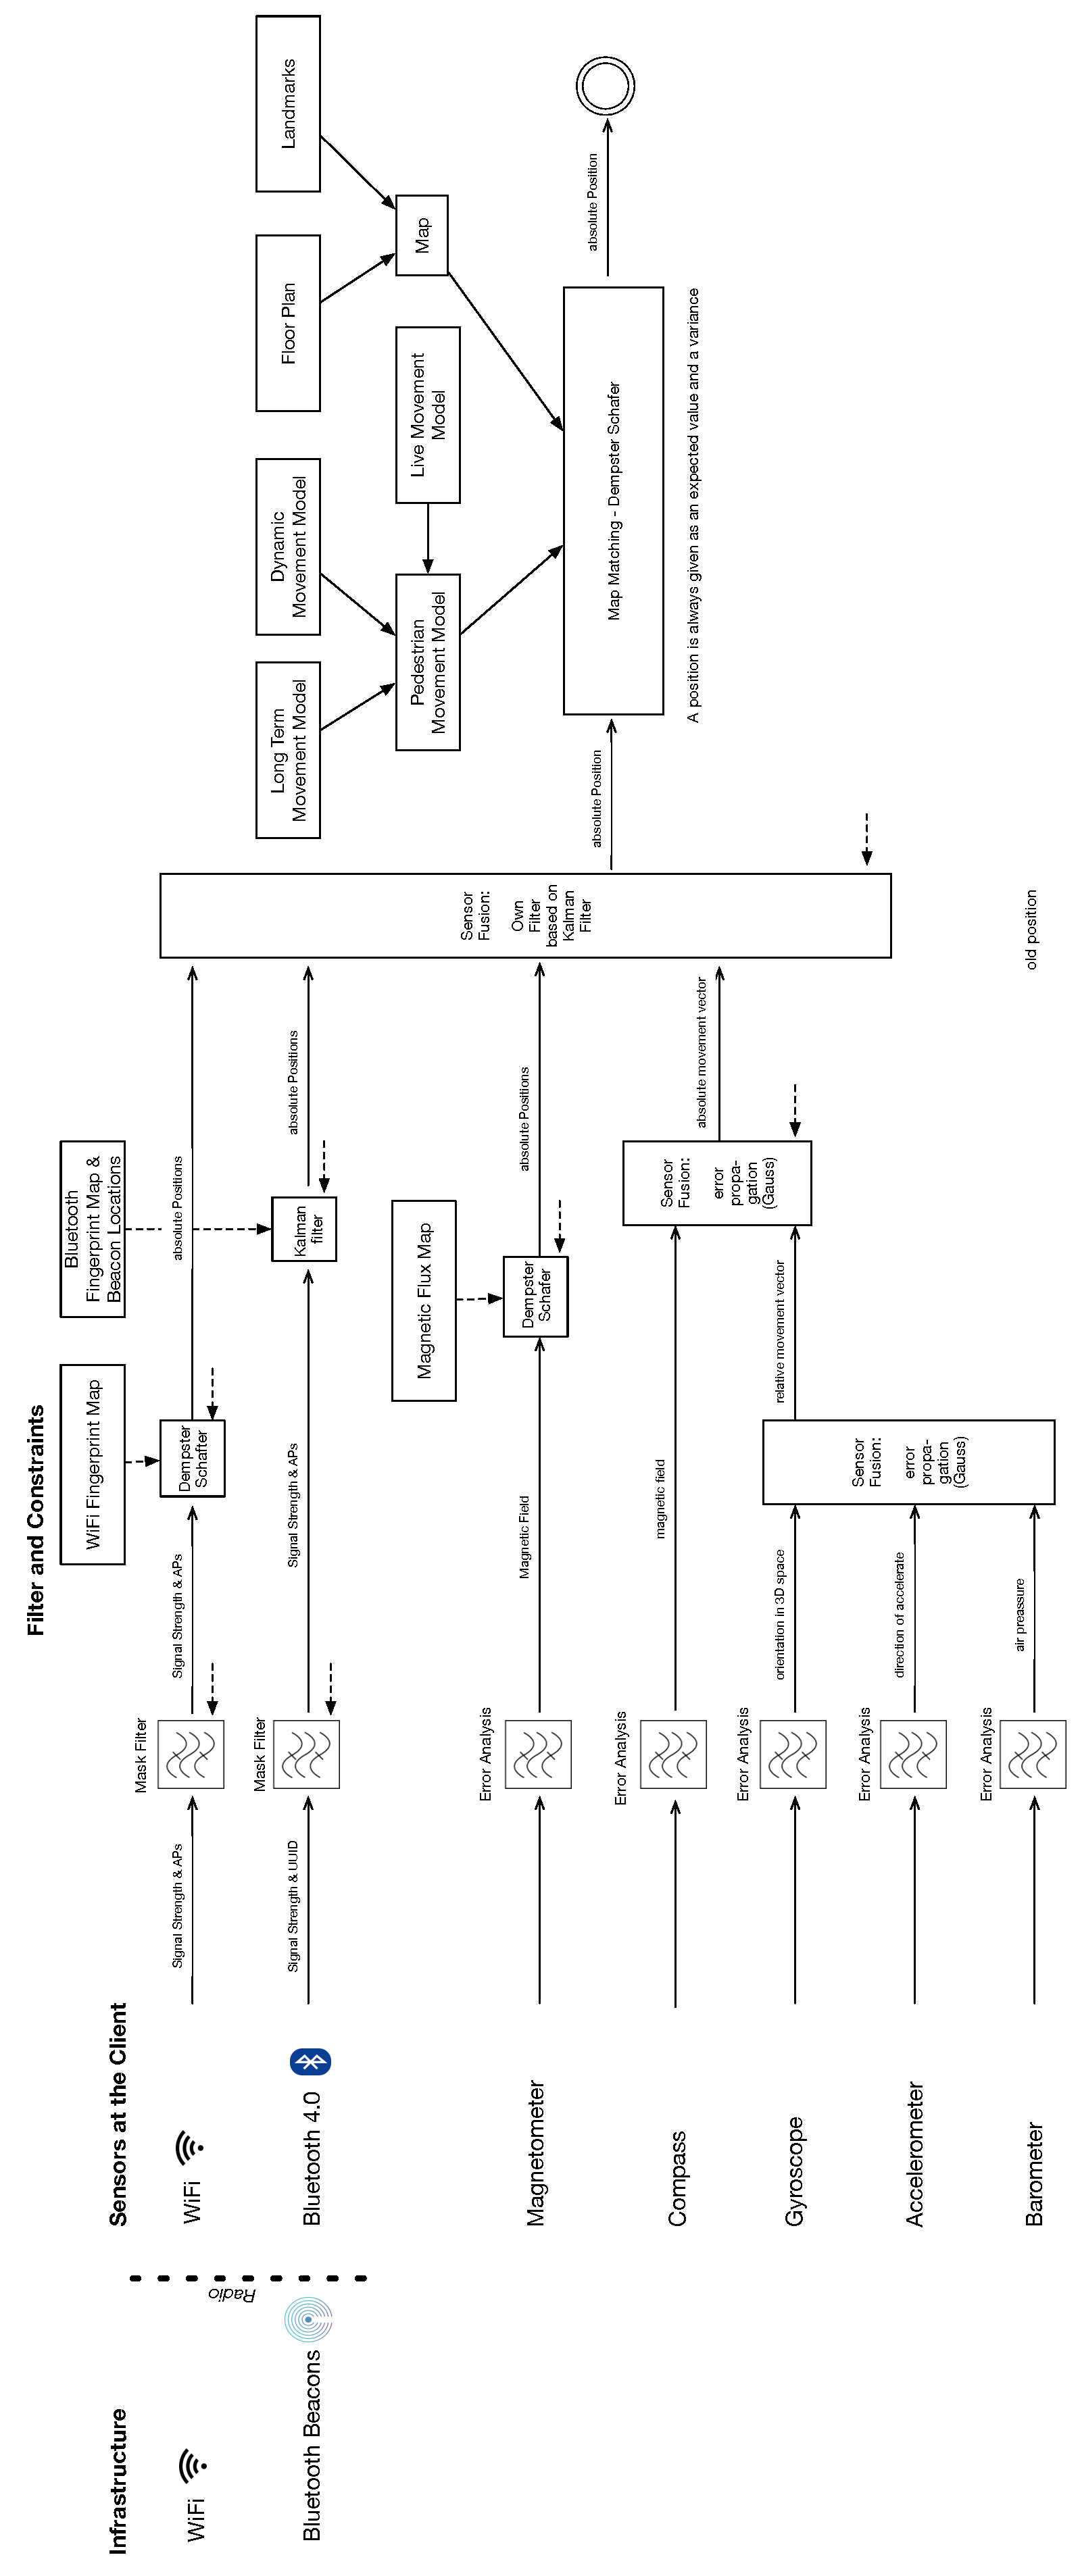
\includegraphics[width=0.6\textwidth]{images/Final_Positioning_system.pdf}
	\caption{Concept of a new Indoor Positioning System}
	\label{fig:ips}
\end{figure}

In figure \ref{fig:ips} the model is shown. The infrastructure contains WiFi Access Points and Bluetooth. In the most buildings Wifi is already provided and no additional infrastructure has to be deployed. By just monitoring signal strength and access points no direct communication between AP and Client needs to be established. Signal strength and access points in reachable range enable us to use fingerprinting. It is not possible to use energy of the direct path and the Time of Flight of direct path calculations without communication between client and AP. 
The measured signals strengths from different access points are filtered by a modified mask filter - like the one for GPS explained in section \ref{sec:error} - and flagged if they can be identified as unreliable.

After enough measurements to ($>30$) for each AP have been collected a Dempster Schafer is applied to combine the measurements with the WiFi Fingerprint map and the previous position - as output an absolute position in form of an expected value $\mu$ and the associated variance $\sigma^2$ for every dimension is given.

Unlike for WiFi, Bluetooth beacons need to be installed in the infrastructure. However Bluetooth beacons are working with Buetooth Low Energy and are able to work with batteries for longer time. There are two major advantages of using both Bluetooth and Wifi. First the technologies complement each other and improve overall positioning, second they backup each other. Thus devices with disabled Bluetooth or WiFi are still able to calculate acceptable positioning information. Additional devices not supporting Bluetooth 4.0 are able to locate themselves.
The received Bluetooth signals are marked by a mask filter and afterwards interpreted using a Kalman filter and a corresponding Bluetooth fingerprint map. (Kalman filter is used here to take advantages of Kalman and Demster Shafer if both Bluetooth and WiFi is available) Again the output would be an absolute position. 

We decided to not use GPS, ZigBee or Locata in first place since GPS is to unreliable indoors and the average moblie device does not support ZigBee or Locata. 
Even if the LED solution could enhance the systems performance especially to differentiate between different floors in the same design we decided us against it because of an big overhead on development of non reusable components for the initial solution.

The magnetometer could improve the performance and would not increase development effort too much. The principle applied is the same as it is for WiFi and Bluetooth. Therefore all fingerprint maps can be generated at once. For the first filtering to smooth the sensor data we want do use error analysis and throw out outliers. The matching of the measured information to the magnetic flux map again is done using a Kalman filter.

All of the described above strategies are ranging between 1 and 2m accuracy. The output of each sensor interpretation is already a position on a map. The internal sensors Gyroscope, Accelerometer Barometer and Compass need to be interpreted to derive a movement vector which then can be applied to the previous position to calculate an absolute position.

As a first step to get an relative movement vector the signals of Accelerometer, Gyroscope and Barometer are taken. The Gyroscope gives the orientation in 3D space. Combined with the information of the accelerometer - which gives the direction of accelerate it is possible to calculate the direction of accelerate relative to a horizontal plane. Using the air pressure change the direction of the vector can be refined by means of angel to the plane. The relative movement vector (relative to the phones alignment orthographic projected onto the plane) can then be transformed into an absolute vector using the compass. This sensor fusion should be done using the principle of error propagation. 

At this point there are four absolute positions derived using the different technologies which need to be combined. For this combination we decided to develop an own algorithm. The thoughts behind this decision are that all four positions will have different reliabilities which will be visible after testing. An implementation of the Kalman filter is not able to learn - or react to some at this moment unknown coherences but a modified version using a Kalman filter combine with a Bayesian network or even OneR-Algorithem known from Data Mining could fit our purpose. However the decision how to fuse these four given positions the best way could only be made after some field experiments and will be part of future work.

For Map Matching we decided to include different constraints. At first there are the Floor-plan and maybe highlighted and maybe dynamic landmarks. These two maps are combined just by putting one on top of the other. Then there are the movement models. All three movement models can be seen as heat-maps with hot areas with a lot of human traffic and cold areas where humans are less often. The long term movement model is generated using all tracked movement data of a long run (like a bulb exposure in photography). The dynamic movement model can be subject of different rules; Thus if there are patterns detected referencing different times of days in a week (e.g. every saturday at 10.00 till 18.00 o Clock high density of people) this patterns can be modeled in heat-maps again loaded at the expected time. The Live movement Model includes the accumulated data of a short time period. All three movement models are combined building the sum for each position with weights ($p_{ij}=x*long_{ij}+y*dyn_{ij}+z*live_{ij}$ where $i$ and $j$ are the coordinates defining a position and $x$, $y$ and $z$ are the weights). 
The weights cannot be define at this stage of the work. They will be subject of futur work again.

After the Pedestian Movement model and the Map are generated they both are combined in one step using Dempster-Schafer. To do so, for all positions considerable the plausibility is calculated using the Map and the Movement Model to find doubt for specific position. 

To underline the decisions made in the concept we shortly summarize advantages and disadvantages of the design.

\subsubsection{Advantages and Disadvantages}
At this point we will discuss the concept again and measure ourself on the earlier defined measurements. 

Trustworthiness at this point is easy to answer. Our solution will enable every device to locate itself after initially loading the available constraints from a central service. After this has been done no further communication - including forwarding location information - to the system provider is necessary. Thus the whole system is able to run without any feedback data from the user except the pedestrian movement model. This movement model however could be generated with highly accumulated and anonymized data colleced from users willing to share information. In summary we won't expect any trustworthiness issues since "privacy by design" is part of the concept.

Accuracy is at this point unknown but we expect to be able to allow positioning with accuracy below $1.5m$. This looking at the accuracy of the compareable solutions of infsoft and Navizon of $1m$ this is our pessimistic guesstimate. An optimistic value is $<1m$ and our goal for further developments. One advantage of the described concept regarding accuracy is that in all stages measurement errors are propagated and thus no measurement will be lost. All this information is then included into the Map matching process and our unique concept of movement models. Another advantage is that all filters are replaceable and field tests of different realization of the same structure are possible. The corresponding disadvantage is that the development of an optimal solution will need a huge amount of tests and development effort. However the modular structure allows a step by step development with continuous improvements.

Cost efficiency is tried to realize by this stated step by step development and a small working sub-solution. Due to this, the localization will later on work even if WiFi or Bluetooth is turned of.  Additional Hardware will only be needed for the Bluetooth beacons and no infrastructure changes are necessary. In fast moving environments however the effort of generating Fingerprints could be enormous if there are not enough users willing to share their measurements.

At a last step we check which of the chosen use cases are covered.

\subsubsection{Use Cases covered}
With this solution positioning is guarantied and therefor all the focused use cases can be realized. General Indoor Navigation with all its sub use cases, Personalized and Augmented Experience, People and Object tracking by active clients only real life social networks, robotics and more are possible. For proximity marketing the effort would not be in proportion with the return. Location analytics would be possible partly being aware that all very private users are missing in the statistic. 

	\clearpage
% 8 - 12 Seiten
\section{Summary}%conclusion

%gegenpol zu aufgabenstellung, roter faden findet ende mit vergleich(ob und wie anfängliche aufgabenstellung von der arbeit tatsächlich erfüllt wurde) 

	%aufgabenstellung:
		%It seems that hardly any company or vendor makes the approach to be able to connect or controll devices of the competitors in a suitable way. This is the part where this thesis turns up the heat. The content of this thesis deals with smart home solutions and their cross compatibility. First of all basic definitions are clarified then theory is build up to emerge in a middleware solution which connects multiple vendors smart home solutions.	

%wichtigste aussagen des gesammten dokuments erneut nennen und miteinander in beziehung bringen (und bewerten)
%angeben welche pubnkte der arbeit nicht oder nur unzureichend behandelt wurden (schlüssig nachweisen dass es sehr komplex war und deswegen nicht realisierbar in der kruzen zeit, oder sprengt umfang der arbeit)

%auffangbehälter für ungeduldige leser die in der mitte des dokuments aufgehört haben zu lesen

%das wichtigste nochmal in kürze

	Reflecting the path of this thesis the definition of a home successfully led to requirements for smart home technology to actually improve everyday life. Moreover in the scope of this work the Sullivans rule implies that smart home solutions do not have to be fancy. Although some vendors like Samsung rely on feature-ism to maintain sales. This thesis highlights the core needs a smart home solution has to fulfill. Among others Apple HomeKit complies best with these measurements and is therefore chosen as part of the middleware solution.

	The superior solution out of two possible middleware solutions is chosen and implemented. Although the design covers the whole HomeKit api implementation does not. Due to the fact that HomeKit itself is documented well enough and an extra documentation would blast the scope of this thesis. Changes in the device data model in SDPvNext and the IoT Foundation have to be implemented since HomeKit needs meta data like a pairing code which must be stored alongside regular data. The goal of this thesis is to develop a middleware however changes in the two systems that are supposed to be connected are out of scope.\\

\subsection{Reflection}
	%erkenntnisse und ergebnisse

	The elaborated smart home measurements security, smart home functions and cross compatibility are all based on evaluating definitions of smart home and iot as well as basic home functions that nearly everyone can rely to as common sense. By applying these measurements an adequate smart home solution is encountered as part of the middleware solution. To choose the right solutions out of two was tricky business but overall the homebridge solution lost because there is no documentation on the hap protocol which makes implementation nearly impossible.


\subsection{Result}
	Where the middleware solution fulfills its supposed task considering the given limitations of SDPvNext. Future work includes implementing the HomeKit api into the existing middleware but is obsolete until SDPvNext expands its interactivity possibilities to actually control devices over rest. Further tasks include considering large corporation solutions and redefining measurements for their domain.\\

	A big task still remains in the topic of smart home, namely defining official standards. New thesises should cover this topic to actually improve the overall situation inside the world of iot. Another good thread to keep an eye on is the buzzword fog. I guarantee that this as soon as people understand the benefits of this kind of paradigm, big data will get really handy. Further an analysis of user or company driven development trend is predictable. Thank you for reading this thesis!

	%bewertung des ergebnises

	%restrictions um problem mit sdpvnext datamodel erweitern
	%verbesserungen, weitere notwendige schritte, richtung angeben, sonstige anwendungen

	%vergleich mit großkonzern lösungen für weitere arbeit

	%formulierung weiterer aufgabenstellungen und mögliche lösungsansätze


	
	% Anhang
	\clearpage
	\pagestyle{plain}
	\pagenumbering{Roman}
	\setcounter{page}{1}

	%Tabellenverzeichnis
	%\cleardoublepage
	%\phantomsection \label{listoftab}
	%\addcontentsline{toc}{section}{List of tables}
	%\listoftables

	% Quellcodeverzeichnis
	%\cleardoublepage
	%\phantomsection \label{listoflist}
	%\addcontentsline{toc}{section}{Listings}
	%\lstlistoflistings

	% Literaturverzeichnis
	\addcontentsline{toc}{section}{Bibliography}
	\printbibliography
	
	% Glossar
	\setcounter{subsection}{0}
	\addcontentsline{toc}{section}{Appendix}
	\printglossary[style=altlist,title=Glossary]
	
	\cleardoublepage
	


\renewcommand{\thesubsection}{\Alph{subsection}}

\section*{Appendix}







\end{document}
